\documentclass[a4paper, 12pt]{article}
\usepackage{titling}
\usepackage{amsmath}
\usepackage{amssymb}
\usepackage{chngpage}
\usepackage{multirow}
\usepackage{graphicx}
\usepackage{titlesec}
\usepackage{fancyhdr}
\usepackage{chngcntr}
\graphicspath{ {figs/} }
\usepackage{indentfirst}
\usepackage{relsize}
\usepackage[margin=3.7cm]{geometry}
\usepackage{multirow}
\usepackage[table,xcdraw]{xcolor}
\usepackage{hhline}
\usepackage{titletoc}
\usepackage{afterpage}
\usepackage{hyperref, url}
\usepackage{caption} 
\usepackage{float}

\captionsetup[table]{skip=10pt}

\setlength{\droptitle}{-15em}

\titleformat{\chapter}[display]
{\normalfont\bfseries}{}{0pt}{\LARGE}
\titleformat{\section}[display]
{\normalfont\bfseries}{}{0pt}{\LARGE}
\titleformat{\subsection}[display]
{\normalfont\bfseries}{}{0pt}{\Large}
\titleformat{\subsubsection}[display]
{\normalfont\bfseries}{}{0pt}{\large}
\pagestyle{fancy}
\fancyhf{}
\fancyhead[L]{SPECIFIC HEAT OF A SOLID}
\fancyhead[R]{M. de Miguel and Y. Wu}
\fancyfoot[c]{\thepage}

\newcommand\blankpage{%
	\null
	\thispagestyle{empty}%
	\addtocounter{page}{-1}%
	\newpage}


\begin{document}
	\begin{titlepage}
		\centering
		\vfill
		\Large{COMPLUTENSE UNIVERSITY OF MADRID \\ \textbf{FACULTY OF PHYSICAL SCIENCES}}
		\vfill
		\begin{figure}[h!]
			\centering
			
\includegraphics[height=7cm]{cumphysics}
		\end{figure}
		\vfill 
		\textbf{\Large{LABORATORY OF THERMODYNAMICS:}}
		\rule [5pt]{14cm}{2pt}\\
		\LARGE{\textbf{DETERMINATION OF THE SPECIFIC HEAT OF SOLIDS}} \\
		\rule [8pt]{14cm}{2pt}\\
		\vfill
		\vfill
		\vfill
		\vfill
		
		\large{Mario de Miguel Domínguez and YanRu Wu Jin\\ Bachelor's Degree in Physics, 2\textsuperscript{nd} Year, Group 14\\ Experience date: 23\textsuperscript{rd} of March, 2022\\ Delivery date: 30\textsuperscript{th} of March, 2022}
		\vfill
		\vfill
		\vfill
		\vfill
		
		\afterpage{\blankpage}
	\end{titlepage}
	
	\makeatletter
	\thispagestyle{empty}
	\addtocounter{page}{-1}
	\let\latexl@section\l@section
	\def\l@section#1#2{\begingroup\let\numberline\@gobble\latexl@section{#1}{#2}\endgroup}
	\let\latexl@subsection\l@subsection
	\def\l@subsection#1#2{\begingroup\let\numberline\@gobble\latexl@subsection{#1}{#2}\endgroup}
	\let\latexl@subsubsection\l@subsubsection
	\def\l@subsubsection#1#2{\begingroup\let\numberline\@gobble\latexl@subsubsection{#1}{#2}\endgroup}
	\makeatother
	\tableofcontents	
	\thispagestyle{empty}
	\afterpage{\blankpage}
	\newpage
	\section{1 Introduction}
	This assignment aims at the determination of the specific heat of solid substances. More precisely, the specific heat of metallic solids (aluminium, brass and steel) is to be studied at both high and low temperatures.
	The ``high" temperature is set to be the room temperature whereas the ``low" temperature shall be that of the boiling point of liquid nitrogen. \\
	
	The data to be gathered shall help check the validity of the Dulong-Petit law.
	\section{2 Theoretical basis}
	The Zeroth Law of Thermodynamics states that two systems at thermal contact, both envolved in an adiabatic enclosure, evolve to reach thermal equilibrium i.e. the same average temperature for both systems by either emitting or absorbing heat. \\
	
	Moreover, the law of Dulong and Petit states the molar heat capacity of most solids at high temperatures are fairly similar and noticeably close to the value of $3R$. At low temperatures, however, Debye's law shows the heat capacity of these substances are proportional to the cube of their temperatures \textsuperscript{[1]}.
	
	\section{3 Material and experimental method}
	\subsection{3.1 Material}
	\begin{itemize}
		\item Calorimeter
		\item Samples: Aluminium, brass, steel
		\item Gripper
		\item Thermometer
		\item Balance
		\item Liquid N\textsubscript{2}
	\end{itemize}
	\subsection{3.2 Experimental Method}
	\subsubsection{3.2.1 High temperatures}
	Firstly the heat capacity of the calorimeter is to be found. This can be performed by evaluating the final temperature ($T_M$) of a mixture of known masses of cold water ($m_C$) and hot water ($m_H$) at known temperatures ($T_C$ and $T_H$, respectively). \\
	
	All these data known, the specific heat of the calorimeter can be found to be 
	\begin{equation}\label{ccalorimeter}
		C = \frac{m_H (T_H - T_M) - m_C (T_M - T_C)}{T_M - T_C} c_{p_{H_2O}},
	\end{equation}
	being $c_{p_{H_2O}}$ the specific heat of water (4184 J kg\textsuperscript{-1} K\textsuperscript{-1})\textsuperscript{[2]}. \\
	
	To proceed with the determination of the differrent $c_{p_i}$ of the solids, it is of use to measure the mass of the samples. The samples are then immersed (one at a time) in a beaker with water, and then heated up to the boiling point of water. This temperature $T_B$ is measured.  The content of the calorimeter is replaced by cold water ($m'_C, T'_C$) meanwhile, before putting the samples inside. The calorimeter is then covered with the lid and the liquid is stirred until reaching a stable temperature $T'_M$. Then, using the same reasoning as before:
	\begin{equation}\label{cpsolidhot}
		c_p = \frac{m'_C c_{p_{H_2O}} (T'_M - T'_C) + C(T'_M - T'_C)}{m_S (T_B - T'_M)}.
	\end{equation}
	It is proceeded likewise for the three metals.
	\subsubsection{3.2.2 Low temperatures}
	The procedure is similar as that in section 3.2.1, but now the samples shall be immersed in liquid nitrogen. Now it must be considered the N\textsubscript{2} mass loss due to vaporisation. \\
	
	About 400 g of liquid N\textsubscript{2} are poured in the calorimeter, it kept on the balance. 10 pairs of time-mass data are noted and fitted to a linear expression. Then the sample to study (at room temperature) is carefully introduced in the calorimeter. This sudden heating of the nitrogen will make it lose mass at a rather non-linear rate, until the sample reaches the boiling temperature of N\textsubscript{2}. The evaporated N\textsubscript{2} mass associated to the sample cooling shall be
	\begin{equation}\label{masscool}
		m_v = at_b + b + m_s - m_b
	\end{equation}
	$a, b$ being the fit parameters of the normal vaporisation, $m_s$ the mass of the sample and $m_b$ the mass of the system after the bubbling interruption. The heat  emitted by the solid is that needed to evaporate the $m_v$ of N\textsubscript{2}. One can then define
	\begin{equation}\label{cpsolidcold}
		m_s (c_p)_m (T_{amb} - T_{N_2}) = m_v \Delta H_v,
	\end{equation}
	being $T_{amb}$ the room temperature, $T_{N_2}$ that of the boiling of nitrogen (77.35 K) and $\Delta h_v$ the enthalpy of vaporisation of nitrogen (200 J/g) \textsuperscript{[3]}.
	\section{4 Results and questions}
	This section is aimed at presenting the obtained results as well as answering the questions proposed in the assignment script. For further information on the gathered data or the computation of errors, please refer to the correspondent sections in the appendix.
	\subsection{4.1 Question 1}
	We know the whole system is adiabatic, this means there is no net heat transfer between the system and its environment:
	\begin{equation}
		dQ = 0 \nonumber,
	\end{equation}
	but, from the definition of $Q$, we know
	\begin{align*}
		dQ &= dQ_C + dQ_H + dQ_{cal} = m_C c_{p_{H_2O}} dT_C + m_H c_{p_{H_2O}} dT_H + C dT_{cal}  \implies \\ 
		0 &= m_C c_{p_{H_2O}} (T_M - T_C) + m_H c_{p_{H_2O}} (T_M - T_H) + C (T_M - T_H) \implies \\
		C &= -\frac{m_C c_{p_{H_2O}} (T_M - T_C) + m_H c_{p_{H_2O}} (T_M - T_H)}{T_M - T_C}  \implies \\
		C & = c_{p_{H_2O}} \frac{m_H  (T_H - T_M) - m_C (T_M - T_C)}{T_M - T_C}.
	\end{align*}\\

	Notice that both the calorimeter and the cold water are absorbing heat ($dQ_{cal}, \mbox{ } dQ_C > 0$) while the hot water emits heat ($dQ_H < 0$), this forcing $dT_{cal}, \mbox{ } dT_C > 0$ and $dT_H < 0$. \\
	
	In a similar manner, when the pieces of metal are introduced in the system,
	
	\begin{align*}
		dQ &= dQ_C + dQ_S + dQ_{cal} = m'_C c_{p_{H_2O}} dT_C + m_S c_p dT_S + C dT_{cal} \implies \\
		0 &= m'_Cc_{p_{H_2O}}(T'_M - T'_C) + m_S c_p (T'_M - T_B) + C(T'_M - T'_C) \implies \\
		c_p &= -\frac{m'_Cc_{p_{H_2O}}(T'_M - T'_C) + C(T'_M - T'_C)}{m_S(T'_M - T_B)} \implies \\
		c_p &= \frac{m'_Cc_{p_{H_2O}}(T'_M - T'_C) + C(T'_M - T'_C)}{m_S(T_B - T'_M)} 
	\end{align*}.\\

	Again, the solid is emitting heat ($dQ_{S} < 0 \implies dT_S < 0$) and the calorimeter and the cold water absorb it ($dQ_C, \mbox{ } dQ_{cal} > 0 \implies dT_C, \mbox{ } dT_{cal} > 0$).
	\subsection{4.2 Question 2}
	The heat capacity has been estimated following the procedure described in section 3. Table 1 displays the collected values for the mass and temperatures of the added hot and cold water. \\
	
	Notice that the water masses have not been weighed directly but found as a difference of masses: $m_C$ is the difference of the calorimeter mass before and after adding the cold water and $m_H$ has been computed as the mass difference after adding the hot water to the calorimeter.\\
	
	\begin{table}[h!]
		\centering
			\caption{Content measurements to estimate the $C$ of the calorimeter}
		\begin{tabular}{| c | c | }
			\hline
			\textbf{Cold water mass $\boldsymbol{m_C}$ (g)} & 246.50 $\pm$ 0.14 \\
			\hline	
			\textbf{Hot water mass $\boldsymbol{m_H}$ (g)} & 203.10 $\pm$ 0.14 \\
			\hline	
			\hline
			\textbf{Cold water temperature $\boldsymbol{T_C}$ (ºC)} & 21.10 $\pm$ 0.05 \\
			\hline	
			\textbf{Hot water temperature $\boldsymbol{T_H}$ (ºC)} & 79.00 $\pm$ 0.05 \\
			\hline	
			\textbf{Final temperature $\boldsymbol{T_M}$ (ºC)} & 45.10 $\pm$ 0.05 \\
			\hline	
		\end{tabular}

\end{table} 

	From this data, and with help of equations \ref{ccalorimeter} and \ref{dccalorimeter}, one may find $C$ to be
		\begin{equation*}\label{rccalorimeter}
			C = 168.9 \pm 5.4\mbox{ J/ºC} = 168.9 \pm 5.4\mbox{ J/K}
		\end{equation*}
	
	From here the equivalent in water $m_w$ is fairly easy to estimate. From the definition of specific heat capacity $c_p$
	\begin{equation}\label{meqwater}
		c_p = \frac{Q}{m\Delta T} \equiv \frac{C}{m} \implies m_w = \frac{C}{c_{p_{H_2O}}},
	\end{equation}
	being $c_{p_{H_2O}}$ the specific heat of water. Therefore
	\begin{equation*}\label{rmeq}
		m_w = 40.4 \pm 1.3 \mbox{ g}
	\end{equation*}

	\subsection{4.3 Question 3}
	Known the $C$ of the calorimeter, it is simple to compute the specific heat capacity of the solids. The solids shall be referred as solid 1, solid 2 and solid 3 for the moment. The experiment has been performed at different conditions for each solid, hereby displayed:
	\begin{itemize}
		\item Solid 1: \\
		
		\begin{table}[h!]
			\centering
			\caption{Experience with solid 1}
			\begin{tabular}{|c|c|}
				\hline
					\textbf{Cold water mass $\boldsymbol{m'_{C_1}}$ (g)} & 268.60 $\pm$ 0.14 \\
				\hline
					\textbf{Solid mass $\boldsymbol{m_{s_1}}$ (g)} & 89.5 $\pm$ 0.1 \\
				\hline
				\hline
					\textbf{Cold water temperature $\boldsymbol{T'_{C_1}}$ (ºC)} & 20.60 $\pm$ 0.05 \\
				\hline
					\textbf{Solid temperature when put in the calorimeter $\boldsymbol{T_{B_1}}$ (ºC)} & 98.00 $\pm$ 0.05 \\
				\hline
					\textbf{Final temperature $\boldsymbol{T'_{M_1}}$ (ºC)} & 25.10 $\pm$ 0.05 \\
				\hline
			\end{tabular}
		
		\end{table}
		Equation \ref{cpsolidhot} yields the following result for these data:
		\begin{equation*}\label{rsolid1}
			c_{p_1} = 0.891 \pm 0.015\mbox{ J g\textsuperscript{-1} K\textsuperscript{-1} }
		\end{equation*}
		\item Solid 2: \\
		
		\begin{table}[h!]
			\centering
				\caption{Experience with solid 2}
			\begin{tabular}{|c|c|}
				\hline
				\textbf{Cold water mass $\boldsymbol{m'_{C_2}}$ (g)} & 256.00 $\pm$ 0.14 \\
				\hline
				\textbf{Solid mass $\boldsymbol{m_{s_2}}$ (g)} & 88.8 $\pm$ 0.1 \\
				\hline
				\hline
				\textbf{Cold water temperature $\boldsymbol{T'_{C_2}}$ (ºC)} & 22.50 $\pm$ 0.05 \\
				\hline
				\textbf{Solid temperature when put in the calorimeter $\boldsymbol{T_{B_2}}$ (ºC)} & 98.00 $\pm$ 0.05 \\
				\hline
				\textbf{Final temperature $\boldsymbol{T'_{M_2}}$ (ºC)} & 24.90 $\pm$ 0.05 \\
				\hline
			\end{tabular}
		
		\end{table}
	
		This evaluated with equation \ref{cpsolidhot}, one may obtain:
		\begin{equation*}\label{rsolid2}
			c_{p_2} = 0.458 \pm 0.014\mbox{ J g\textsuperscript{-1} K\textsuperscript{-1} }
		\end{equation*}
		\item Solid 3:\\
		
		\begin{table}[h!]
			\centering
			\caption{Experience with solid 3}
			\begin{tabular}{|c|c|}
				\hline
				\textbf{Cold water mass $\boldsymbol{m'_{C_3}}$ (g)} & 254.80 $\pm$ 0.14 \\
				\hline
				\textbf{Solid mass $\boldsymbol{m_{s_3}}$ (g)} & 90.7 $\pm$ 0.1 \\
				\hline
				\hline
				\textbf{Cold water temperature $\boldsymbol{T'_{C_3}}$ (ºC)} & 22.50 $\pm$ 0.05 \\
				\hline
				\textbf{Solid temperature when put in the calorimeter $\boldsymbol{T_{B_3}}$ (ºC)} & 98.00 $\pm$ 0.05 \\
				\hline
				\textbf{Final temperature $\boldsymbol{T'_{M_3}}$ (ºC)} & 24.90 $\pm$ 0.05 \\
				\hline
			\end{tabular}
			
		\end{table}
	\end{itemize}


	When substituted in equation \ref{cpsolidhot}, it yields
	\begin{equation*}\label{rsolid3}
		c_{p_2} = 0.407 \pm 0.013 \mbox{ J g\textsuperscript{-1} K\textsuperscript{-1} }
	\end{equation*}
	We may now check the tabulated values of the heat capacities of aluminium, brass, and steel.
	
	\begin{table}[h!]
		\centering
			\caption{Tabulated values for the heat capacities\textsuperscript{[4]}}
		\begin{tabular}{|c|c|}
			\hline
			\textbf{Solid} & $\boldsymbol{c_p}$ \textbf{(J g\textsuperscript{-1} K\textsuperscript{-1}})\\
			\hline
			\textbf{Aluminium} & 0.897 \\
			\textbf{Brass} & 0.385 \\
			\textbf{Steel} & 0.449 \\
			\hline
		\end{tabular}

	\end{table}
	These have been assumed to have an uncertainty of 10\textsuperscript{-3} J g\textsuperscript{-1} K\textsuperscript{-1}. It can be seen that aluminium corresponds to solid 1, brass to solid 3 and steel to solid 2.
	If we were to check the law of Dulong-Petit, we just need to find the molar mass of the compounds, these being, in g/mol, $mm_{Al} = 26.982,\mbox{ } mm_{Steel} \approx mm_{Fe} = 55.845 $ and $mm_{Brass} \approx mm_{Cu} = 63.546$. Considering $\bar{c_p} = c_p \cdot mm$:
	
	\begin{table}[h!]
		\centering
			\caption{Experimental molar heat capacities}
		\begin{tabular}{|c|c|}
			\hline
			\textbf{Solid} & $\boldsymbol{\bar{c_p}}$ \textbf{(J mol\textsuperscript{-1} K\textsuperscript{-1}})\\
			\hline
			\textbf{Aluminium} & 24.04 $\pm$ 0.40 \\
			\textbf{Brass} & 25.83 $\pm$ 0.81\\
			\textbf{Steel} & 25.59 $\pm$ 0.78\\
			\hline
		\end{tabular}
	
	\end{table}

	These results are fairly satisfactory, as  according to Dulong-Petit law these values should approach 25 $\frac{\mbox{J}}{\mbox{mol K}}$. 
	\subsection{4.4 Question 4}
	Equations \ref{dccalorimeter} and \ref{dcp} may be considered to be the addition in quadrature of several terms, each of them depending being the consequence of the uncertainty of one of the quantities used to find the values of $C$ or $c_p$. These terms have the form $\frac{\partial C}{\partial Y} \Delta Y$ in the case of the calorimeter heat capacity uncertainty or $\frac{\partial c_p}{\partial Y} \Delta Y$ when considering the uncertainty of the specific heats.\\
	
	Let us start with the analysis of the $C$ formula. One may gather the following terms:\\
	\begin{align*}
		E_{m_H} &= \frac{(T_H - T_M)}{T_M - T_C}\Delta m_H \\
		E_{m_C} &= \Delta m_C \\
		E_{T_H} &= \frac{m_H \Delta T_H}{T_M - T_C} \\
		E_{T_M} &= \frac{m_H + m_C + m_W}{T_C - T_M}\Delta T_M \\
		E_{T_C} &= \frac{m_C + m_W}{T_M - T_C}\Delta T_C
	\end{align*}

	Notice that all these terms should be multiplied by $c_{p_{H_2O}}$, but we do not need to consider this factor for our current computation. \\
	
	We may find \\
	\begin{align*}
		E_{m_H} &= 0.20 \mbox{ J/K}\\
		E_{m_C} &= 0.15 \mbox{ J/K}\\
		E_{T_H} &= 0.42 \mbox{ J/K}\\
		E_{T_M} &= -1.02 \mbox{ J/K}\\
		E_{T_C} &= 0.60 \mbox{ J/K}\\
	\end{align*} 
	Since these terms are being added in quadrature, we are interested in their absolute values, so it can be seen that the mixture temperature $T_M$ is the one that influences most the quantity uncertainty. \\
	
	Proceeding in a similar way with expression \ref{dcp}, one may find the following term:
	
	\begin{align*}
		E_{m'_C} &= \frac{c_{p_{H_2O}} (T'_M - T'_C)}{m_S(T_B - T'_M)}\Delta m'_C \\
		E_{m_S} &= \frac{c_p \Delta m_S}{m_S} \\
		E_{T'_C} &= \frac{C + m'_c c_{p_{H_2O}} }{m_S (T'_M - T_B)}\Delta T'_C \\
		E_{T_B} &= \frac{c_p \Delta T_B}{T_B - T_M'} \\
		E_{T'_M} &= \frac{m'_C c_{p_{H_2O}} + C + m_S c_p}{m_S(T_B - T'_M)}\Delta T'_M \\
		E_{C} &= \frac{T'_M - T'_C}{m_S(T_B - T'_M)}\Delta C
	\end{align*}
	
	which, substituting the data in section tables 2, 3 and 4, become: \\
	\begin{table}[h!]
		\centering
		\caption{Term effects on the $\Delta c_p$ results (J g\textsuperscript{-1} K\textsuperscript{-1})}	
		\begin{tabular}{|c|c|c|c|}
			\hline
				& \textbf{Aluminium} & \textbf{Brass} & \textbf{Steel} \\
			\hline
			$E_{m'_C}$ & 0.00041 & 0.00019 & 0.00022 \\
			$E_{m_S}$ & 0.00100 & 0.00045 & 0.00052 \\
			$E_{T'_C}$ & -0.00990 & -0.00884 & -0.00955 \\
			$E_{T_B}$ & 0.00061 & 0.00026 & 0.00031 \\
			$E_{T'_M}$ & 0.01051 & 0.00910 & 0.00986 \\
			$E_{C}$ & 0.00369 & 0.00176 & 0.00198 \\
			\hline
		\end{tabular}
		
	\end{table}

	As seen in table 7, it is again the equilibrium temperature ($T'_M$ in this case) that makes the largest effect in the final error, regardless of the studied substance.
	\subsection{4.5 Question 5}
	According to the measurements displayed in section A.1 in the appendix, the vaporisation of nitrogen by the outside air has been found to follow the regression lines:
	
	\begin{align}
		m &= -(0.04277 \mp 0.00015)t + (239.2049 \pm 0.0048)  \mbox{ (before introducing aluminium).} \\
		m &= -(0.03283 \mp 0.00015)t + (160.164 \pm 0.011) \mbox{ (before introducing steel).} \\
		m &= -(0.02683 \mp 0.00026)t + (115.510 \pm 0.010) \mbox{ (before introducing brass).}
	\end{align}
	 Considering the room temperature to be of 21.5 $\pm$ 0.1 ºC and knowing the mass of the system at the moment it reaches the equilibrium, the vaporised $m_v$ by the metals may be estimated. 

		\begin{table}[h!]
			\centering
			\caption{Mass magnitudes}
			\begin{tabular}{| c | c | c | c | c |}
				\hline
				& $\boldsymbol{m_S}$ \textbf{(g)} & $\boldsymbol{t_b}$ \textbf{(s)} & $\boldsymbol{m_b}$ \textbf{(g)} & $\boldsymbol{m_v}$ \textbf{(g)} \\
				\hline
				\textbf{Aluminium} & 88.54 $\pm$ 0.02 & 150.1 $\pm$ 5.0 & 252.22 $\pm$ 0.02 & 69.20 $\pm$ 0.22\\
				\textbf{Brass} & 89.48 $\pm$ 0.02 & 170.1 $\pm$ 5.0 & 170.44 $\pm$ 0.02 & 29.99 $\pm$ 0.14\\
				\textbf{Steel} & 89.04 $\pm$ 0.02 & 160.1 $\pm$ 5.0 & 207.72 $\pm$ 0.02 & 36.23 $\pm$ 0.18\\
				\hline
			\end{tabular}
		
		\end{table}
	All these magnitudes can be evaluated in equation \ref{cpsolidcold} to find the values:
		\begin{table}[h!]
		\centering
		\caption{Experimental values for the heat capacities at cold temperatures}
		\begin{tabular}{|c|c|}
			\hline
			\textbf{Solid} & $\boldsymbol{(c_p)_m}$ \textbf{(J g\textsuperscript{-1} K\textsuperscript{-1}})\\
			\hline
			\textbf{Aluminium} & 0.7193 $\pm$ 0.0043 \\
			\textbf{Brass} & 0.3084 $\pm$ 0.0021 \\
			\textbf{Steel} & 0.3744 $\pm$ 0.0026 \\
			\hline
		\end{tabular}
		
	\end{table}

	 Notice the mass of the samples is not the same as those in the experience at high temperatures, for other samples made of the same materials have been used. 
	 \subsection{4.6 Question 6}
	 
	 The molar heat capacities at low temperatures, these are not what they should, according to Dulong-Petit law. Recall that this precicted heat capacities to be of about 25 J mol\textsuperscript{-1} K\textsuperscript{-1}. This can be seen to be fairly accurete when it comes to the high temperature results (Table 6). Nonetheless, when it comes to the results at low temperatures this approximation is not fulfilled, but instead one finds\\
	% \newpage
	 \begin{table}[h!]
	 	\centering
	 	\caption{Experimental molar specific heats}
	 	\begin{tabular}{|c|c|}
	 		\hline
	 		\textbf{Solid} & $\boldsymbol{\bar{c_p}}$ \textbf{(J mol\textsuperscript{-1} K\textsuperscript{-1}})\\
	 		\hline
	 		\textbf{Aluminium} & 19.41 $\pm$ 0.11 \\
	 		\textbf{Brass} & 19.60 $\pm$ 0.14\\
	 		\textbf{Steel} & 20.91 $\pm$ 0.15\\
	 		\hline
	 	\end{tabular}
	 	
	 \end{table}
	 
	 So it can be seen the heat capacities are lower than predicted bu Dulong-Petit law.\\
	 
	 At low temperatures solids stop following the Dulong-Petit law, but behave in terms of Debye's instead. The latter may be cast as:
	 \begin{equation}\label{Debyelaw}
	 	\overline{(c_p)_m} = \frac{12R\pi^4}{5} \left(\frac{T}{T_D}\right)^3,
	 \end{equation}
	 where $T_D$ is the Debye temperature of each material.\\
	
	Since the Debye temperatures $T_D >> T$ in these low temperature regimes. For low temperatures, the Debye temperatures for aluminium, copper and iron are approximately 428, 343 and 470 K, respectively\textsuperscript{[5]}. Let us consider the molar heat capacity Debye's law would yield for brass (copper), as this shall be the highest of the three materials due to its lower Debye temperature.\\
	\begin{equation}\label{approx}
		\overline{(c_p)_m} = \frac{12 \pi^4}{5}\left(\frac{77.35}{343}\right)^3 R \approx 2.64 R < 3R.
	\end{equation}

	So one should expect lower molar hear capacities than those predicted by the Dulong-Petit's law, which is what may be seen in table 9.\\
	\section{5 Conclusion}
	The results are overall accurate and precise, they satisfying the empirical laws of both Dulong-Petit and Debye in each case. Some remarks may be stated. \\
	
	First and foremost, brass and steel have been ``approximated" to be entirely made of copper and iron, respectively. However, one must not forget these are alloys that include other elements, which may alter some quantities such as the compound Debye temperature, its molar mass and consequently its heat capacity. Nonetheless this conjecture has seemed to be good enough when it comes to the results it has yielded. \\
	
	Furthermore, when measuring the heat capacities at low temperatures, the balance was set to save the mass data each five seconds, this dealing to a poor estimation of the moment at which the nitrogen reached equilibrium with the solids. However, even though the time uncertainty was set to be of 5 seconds (noticeably high), this does not seem to have had influenced greatly the values for the heat capacities, they being even more precise than the homologous results for the high temperatures. \\
	
	As a final curiosity, it may be seen in figure 3 (section A.1) the slope of the data points after the brass reaches equilibrium with the nitrogen is steeper than it should. This could be due to the sensitivity of the nitrogen, it evaporating faster just by exhaling hot air close to the system.   
	
	\section{References}
	[1] Kondepudi, D. \& Prigogine, I. (2015). Heat Capacities of Solids. In \textit{Modern thermodynamics: From heat engines to dissipative structures}. Wiley. \\
	
	[2] Wikimedia Foundation. (2022, March 2). \textit{Specific heat capacity}. Wikipedia. Retrieved March 26, 2022, from \url{https://en.wikipedia.org/wiki/Specific\_heat\_capacity}\\
	
	[3] ``Determination of the specific heat of solids" Complutense University of Madrid, 2021.\\
	
	[4] Haynes, W. M. (2015). \textit{CRC Handbook of Chemistry and Physics.} Taylor \& Francis Group. \\
	
	[5] Wikimedia Foundation. (2022, January 26). \textit{Debye model}. Wikipedia. Retrieved March 28, 2022, from \url{https://en.wikipedia.org/wiki/Debye_model}

	\newpage
	\section{Appendix}
	\subsection{A.1 Raw data}
	This section is to gather the obtained data in the second part of the experiment, by making use of the balance software. \\
	
	\tiny{*Tables start at next page since they were too long to fit in this page.}
	%%%ALUMINIUM
	
\newpage
	\begin{table}[hbt!]
		\centering
		\caption{Measurements for the aluminium sample}
		\begin{tabular}{|c | c|}
			\hline
			\textbf{Time (s)} & \textbf{Mass (g)} \\ 
			\hline
		0,0               & 239,20            \\
		10,2              & 238,78            \\
		15,0              & 238,56            \\
		20,0              & 238,34            \\
		25,0              & 238,14            \\
		30,1              & 237,92            \\
		35,1              & 237,70            \\
		40,1              & 237,50            \\
		45,0              & 237,28            \\
		50,0              & 237,06            \\
		\rowcolor[HTML]{FFFF00} 
		55,0              & 320,78            \\
		60,0              & 314,54            \\
		65,1              & 309,16            \\
		70,0              & 304,14            \\
		75,0              & 300,00            \\
		80,1              & 296,32            \\
		85,0              & 292,52            \\
		90,1              & 289,28            \\
		95,0              & 286,00            \\
		100,1             & 282,76            \\
		105,0             & 279,86            \\
		110,0             & 277,04            \\
		115,0             & 274,52            \\
		120,1             & 271,98            \\
		125,0             & 269,42            \\
		130,1             & 267,02            \\
		135,0             & 264,48            \\
		140,1             & 261,16            \\
		145,0             & 255,24            \\
		\rowcolor[HTML]{FFFF00} 
		150,1             & 252,22            \\
		155,0             & 251,92            \\
		160,1             & 251,68            \\
		165,0             & 251,44            \\
		170,0             & 251,20            \\
		175,0             & 250,98            \\
		180,1             & 250,76            \\
		185,0             & 250,56            \\
		190,1             & 250,40           \\
		\hline
	\end{tabular}

\end{table}
	
	%%%BRASS

\newpage
\begin{table}[hbt!]
	\centering
	\caption{Measurements for the brass sample}
	\begin{tabular}{|c | c|}
		\hline
		\textbf{Time (s)} & \textbf{Mass (g)} \\ 
		\hline
		0,0               & 115,50            \\
		10,0              & 115,24            \\
		15,1              & 115,08            \\
		20,0              & 115,00            \\
		25,0              & 114,86            \\
		30,1              & 114,72            \\
		35,1              & 114,58            \\
		40,1              & 114,42            \\
		45,0              & 114,28            \\
		50,0              & 114,16            \\
		55,1              & 114,04            \\
		60,1              & 113,88            \\
		65,1              & 113,78            \\
		\rowcolor[HTML]{FFFF00} 
		70,1              & 201,80            \\
		75,0              & 199,30            \\
		80,1              & 196,82            \\
		85,1              & 194,60            \\
		90,0              & 192,48            \\
		95,1              & 190,58            \\
		100,1             & 188,68            \\
		105,1             & 187,04            \\
		110,0             & 185,46            \\
		115,0             & 183,98            \\
		120,0             & 182,66            \\
		125,0             & 181,38            \\
		130,0             & 180,26            \\
		135,1             & 179,14            \\
		140,0             & 178,12            \\
		145,1             & 177,18            \\
		150,1             & 176,18            \\
		155,0             & 175,32            \\
		160,0             & 174,46            \\
		165,2             & 172,32            \\
		\rowcolor[HTML]{FFFF00} 
		170,1             & 170,44            \\
		175,1             & 170,12            \\
		180,1             & 169,92            \\
		185,0             & 169,60            \\
		190,0             & 169,40            \\
		195,0             & 169,08            \\
		200,1             & 168,88  \\ 
		\hline
	\end{tabular}

\end{table}
\newpage
	
	%%%STEEL
	% Please add the following required packages to your document preamble:
	% \usepackage{booktabs}
	% \usepackage[table,xcdraw]{xcolor}
	% If you use beamer only pass "xcolor=table" option, i.e. \documentclass[xcolor=table]{beamer}
	\begin{table}[H]
		\centering
		\caption{Measurements for the steel sample}
		\begin{tabular}{|c | c|}
			\hline
			\textbf{Time (s)} & \textbf{Mass (g)} \\ 
			\hline
		0,0               & 160,18            \\
		10,1              & 159,84            \\
		15,0              & 159,66            \\
		20,0              & 159,52            \\
		25,0              & 159,32            \\
		30,1              & 159,16            \\
		35,0              & 159,00            \\
		40,1              & 158,84            \\
		45,0              & 158,70            \\
		50,1              & 158,54            \\
		\rowcolor[HTML]{FFFF00} 
		55,0              & 245,86            \\
		60,0              & 242,68            \\
		65,0              & 240,10            \\
		70,1              & 237,52            \\
		75,0              & 235,08            \\
		80,2              & 232,80            \\
		85,1              & 230,72            \\
		90,1              & 228,72            \\
		95,0              & 226,88            \\
		100,1             & 225,10            \\
		105,0             & 223,50            \\
		110,1             & 221,94            \\
		115,0             & 220,56            \\
		120,1             & 219,20            \\
		125,0             & 217,92            \\
		130,1             & 216,70            \\
		135,0             & 215,62            \\
		140,1             & 214,66            \\
		145,0             & 213,64            \\
		150,1             & 210,40            \\
		155,0             & 208,12            \\
		\rowcolor[HTML]{FFFF00} 
		160,1             & 207,72            \\
		165,0             & 207,48            \\
		170,1             & 207,30            \\
		175,0             & 207,12            \\
		180,1             & 206,96            \\
		185,0             & 206,82            \\
		190,1             & 206,68            \\
		195,0             & 206,54            \\
		200,1             & 206,40            \\
		205,0             & 206,24  \\
			\hline
		\end{tabular}

	\end{table}

	\begin{figure}[hbt!]
		\centering
		\caption{Aluminium curve}
		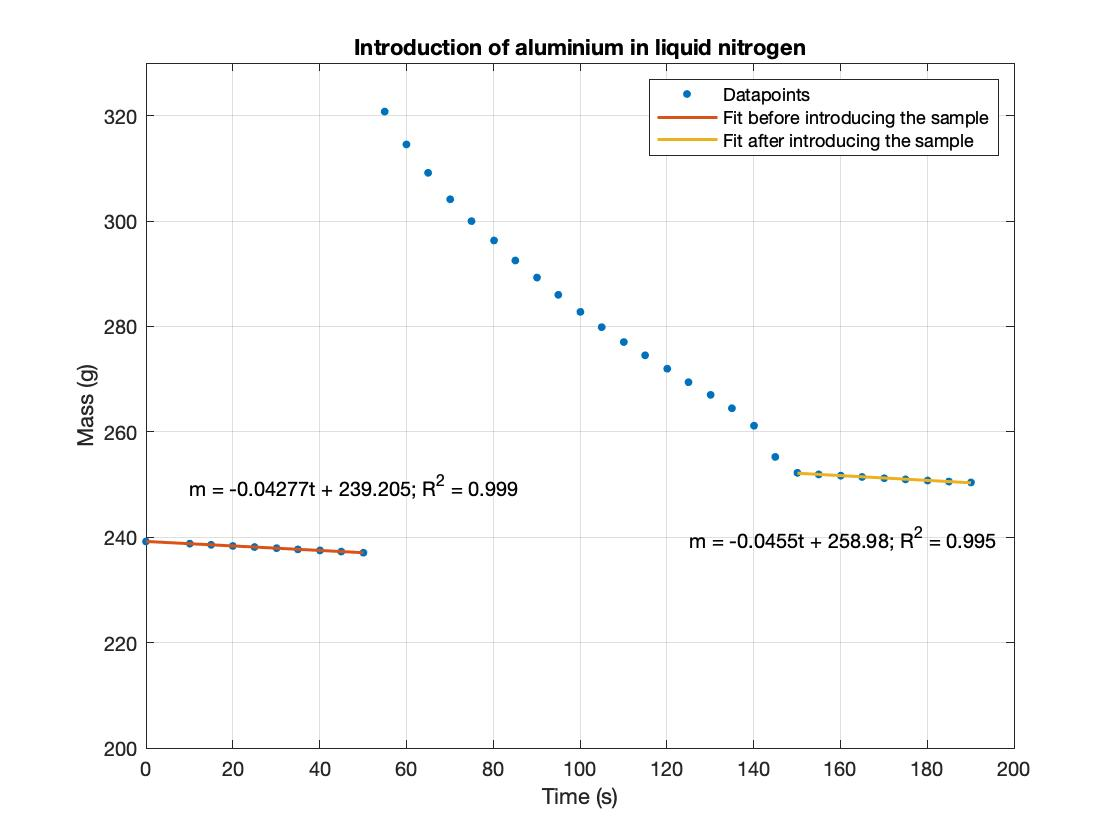
\includegraphics[height=9cm]{aluminiumcurve}
	\end{figure}

	\begin{figure}[hbt!]
		\centering
		\caption{Brass curve}
		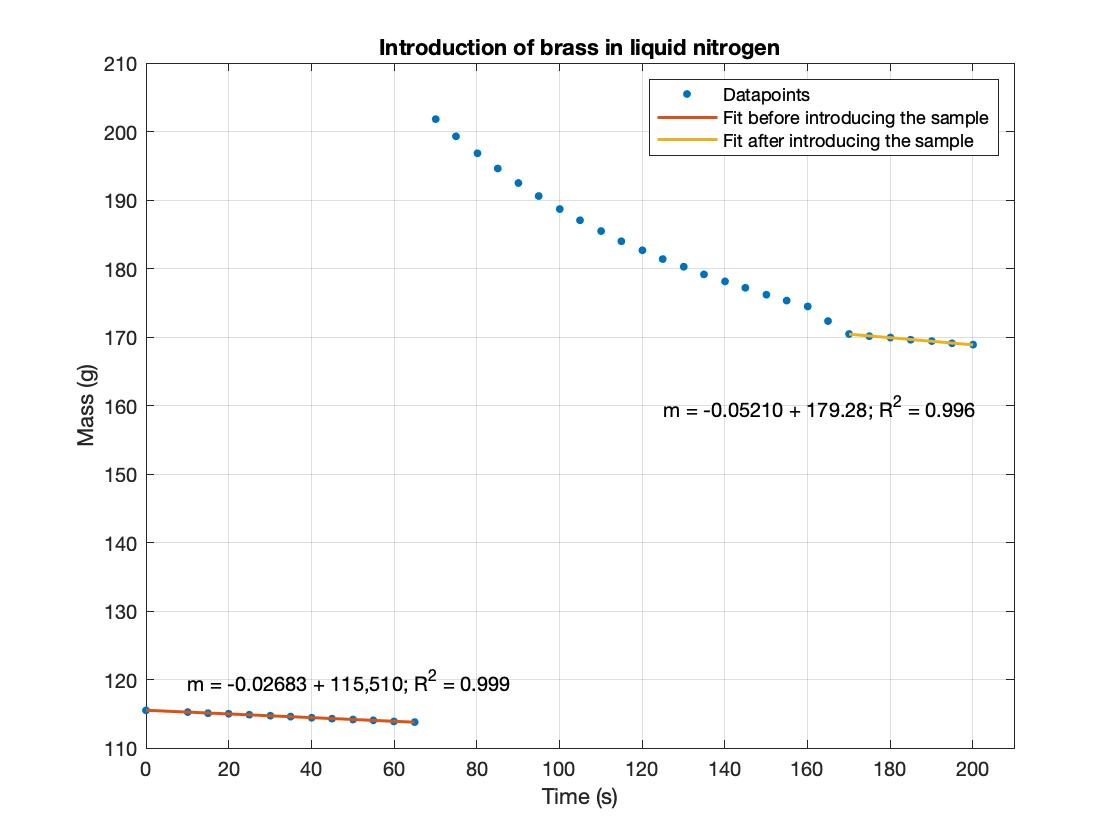
\includegraphics[height=9cm]{brasscurve}
	\end{figure}

	\begin{figure}[hbt!]
		\centering
		\caption{Steel curve}
		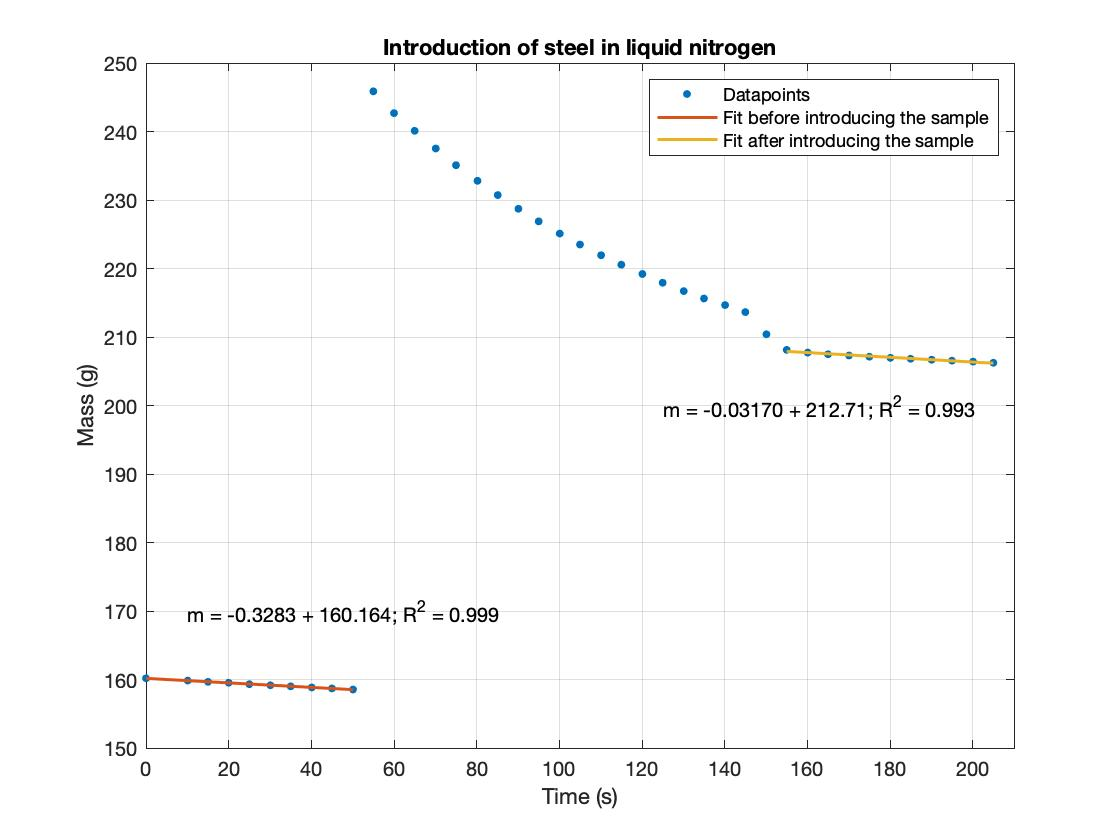
\includegraphics[height=9cm]{steelcurve}
	\end{figure}
\normalsize{}
	\subsection{A.2 Presentation of results}
	Most of the results have been presented in such way to allow easier readability, these not necessarily being in IS units, but multiples of these.\\
	 
	Most results have been presented considering up to two significant figures of their uncertainties, with the exception of values with exact uncertainties.\\
	
	Theoretical errorless values have been presented up to three decimal figures. Percentages are displayed up to two decimal figures.
	\subsection{A.3 Error estimations}
	\subsubsection{A.3.1 Direct measurements}
	The direct errors have been considered those of the precision of the used devices. \\
	
	Some of the tabulated quantities, such as the enthalpy of vaporisation of nitrogen or the theoretical heat capacities have been considered to have errors of precision. Theoretical constants (such as $c_{p_{H_2O}}$) have been treated as errorless quantities. \\
	
	All masses have been measured directly, but the water ones in the first part of the assignment. Time uncertainties have been set to be the space between data points saved by the balance software.\\
	
	No random errors have been computed during the assignment.
	\subsubsection{A.3.2 Indirect measurements}
	\begin{itemize}
		\item Part I: $c_p$ at high temperatures.
		
		*The uncerainty of the water masses has been taken as $\sqrt{0.1^2 + 0.1^2}$ = 0.14 g, as these quantities have been computed as the difference between the calorimeter mass before and after adding each amount of water, each of them having an uncertainty of 0.1 g, i.e. the precision of the used balance.
		\begin{multline}\label{dccalorimeter}
			\Delta C = c_{p_{H_2O}} \sqrt{\left(\frac{(T_H - T_M) \Delta m_H}{T_M - T_C}\right)^2 + (\Delta m_C)^2 + \left(\frac{m_H \Delta T_H}{T_M - T_C}\right)^2} \\ \overline{+ \left(\frac{m_H + m_C + %m_W
					 \frac{C}{c_{p_{H_2O}}}}{T_C - T_M}\Delta T_M\right)^2 + \left(\frac{m_c + %m_W
					 \frac{C}{c_{p_{H_2O}}}}{T_M - T_C}\Delta T_C\right)^2}
		\end{multline}
		\begin{multline}\label{dcp}
		\Delta c_p = \sqrt{\left(\frac{c_{p_{H_2O}} (T'_M - T'_C)}{m_S(T_B - T'_M)}\Delta m'_C \right)^2 + \left(\frac{c_p \Delta m_S}{m_S}\right)^2 + \left(\frac{C + m'_c c_{p_{H_2O}} }{m_S (T'_M - T_B)}\Delta T'_C\right)^2} \\ \overline{+ \left(\frac{c_p \Delta T_B}{T_B - T_M'}\right)^2 + \left(\frac{m'_C c_{p_{H_2O}} + C + m_S c_p}{m_S(T_B - T'_M)}\Delta T'_M\right)^2 + \left(\frac{T'_M - T'_C}{m_S(T_B - T'_M)}\Delta C\right)^2}
		\end{multline}
	\begin{equation}
		\Delta \overline{c_p} = \sqrt{[(c_p)_m\Delta mm]^2 + [mm \Delta (c_p)_m ]^2}
	\end{equation}
	\item Part II: $c_p$ at low temperatures.
\begin{equation}\label{dmvlow}
		\Delta m_v = \sqrt{(t_b\Delta a)^2 + (a\Delta t_b)^2 + (\Delta b)^2 + (\Delta m_s)^2 + (\Delta m_b)^2}
\end{equation}
\begin{equation}
	\Delta (T_{amb} - T_{N_2}) = \sqrt{(\Delta T_{amb})^2 + (\Delta T_{N_2})^2}
\end{equation}
\begin{multline}
	\Delta (c_p)_m = \sqrt{\left(\frac{\Delta H_v \Delta m_v}{m_S(T_{amb} - T_{N_2})}\right)^2 + \left(\frac{m_v\Delta H_v \Delta m_S}{m_S^2(T_{amb} - T_{N_2})}\right)^2 + \left(\frac{m_v\Delta H_v \Delta (T_{amb} - T_{N_2})}{m_S (T_{amb} - T_{N_2})^2}\right)^2 } \\ \overline{+ \left(\frac{m_v\Delta (\Delta H_v)}{m_S(T_{amb} - T_{N_2})}\right)^2}
\end{multline}
\begin{equation}
	\Delta \overline{(c_p)_m} = \sqrt{[(c_p)_m\Delta mm]^2 + [mm \Delta (c_p)_m ]^2}
\end{equation}
	\end{itemize}
\end{document}